% LaTeX template for Artifact Evaluation V20180713
%
% Prepared by 
% * Grigori Fursin (cTuning foundation, France and dividiti, UK) 2014-2018
% * Bruce Childers (University of Pittsburgh, USA) 2014
%
% See example of this Artifact Appendix in
%  * SC'17 paper: https://dl.acm.org/citation.cfm?id=3126948
%  * CGO'17 paper: https://www.cl.cam.ac.uk/~sa614/papers/Software-Prefetching-CGO2017.pdf
%  * ACM ReQuEST-ASPLOS'18 paper: https://dl.acm.org/citation.cfm?doid=3229762.3229763
%
% (C)opyright 2014-2018
%
% CC BY 4.0 license
%

\documentclass[10pt,twocolumn,nocopyrightspace]{sigplanconf}

% preprint      Remove this option only once the paper is in final form.
% 10pt          To set in 10-point type instead of 9-point.
% 11pt          To set in 11-point type instead of 9-point.
% authoryear    To obtain author/year citation style instead of numeric.
\usepackage{fancyhdr}
\usepackage{amsmath}

%% BEGIN PREAMPLE
\usepackage{graphicx}
\usepackage{amsmath}
\usepackage{algorithm}
\usepackage{algorithmic}
\usepackage{amssymb}
\usepackage{url}
%% \usepackage[]{hyperref} %FOR CAMERA READY NO BOOKMARKS!

%% Tables
%\usepackage[table]{xcolor}


\title{Function Merging by Sequence Alignment\vspace{-2em}}
\authorinfo{}

%\authorinfo{\text{Rodrigo Rocha, $\,$ Pavlos Petoumenos}}
%           {University of Edinburgh, UK}
%           {\url{r.rocha@ed.ac.uk}, \url{ppetoume@inf.ed.ac.uk}}

%\authorinfo{Rodrigo C. O. Rocha}
%           {University of Edinburgh, UK}
%           {\url{r.rocha@ed.ac.uk}}
%
%\authorinfo{Pavlos Petoumenos}
%           {University of Edinburgh, UK}
%           {\url{ppetoume@inf.ed.ac.uk}}
%
%\authorinfo{Zheng Wang}
%           {Lancaster University, UK}
%           {\url{z.wang@lancaster.ac.uk}}
%
%\authorinfo{Murray Cole}
%           {University of Edinburgh, UK}
%           {\url{mic@inf.ed.ac.uk}}
%
%\authorinfo{Hugh Leather}
%           {University of Edinburgh, UK}
%           {\url{hleather@inf.ed.ac.uk}}
%\authorinfo{Murray Cole, $\,$ Hugh Leather}
%           {University of Edinburgh, UK}
%           {\url{mic@inf.ed.ac.uk}, \url{hleather@inf.ed.ac.uk}}

\begin{document}
\maketitle

\begin{abstract}
Resource-constrained devices for embedded systems are becoming increasingly important.
In such systems, memory is highly restrictive, making code size in most cases
even more important than performance.
Compared to more traditional platforms, memory is a larger part of the cost and
code occupies much of it. Despite that, compilers make little effort to reduce
code size.
One key technique attempts to merge the bodies of similar functions.
However, production compilers only apply this optimization to identical functions,
while research compilers improve on that by merging the few functions with
identical control-flow graphs and signatures.
Overall, existing solutions are insufficient and we end up having to either increase cost by adding more memory or remove functionality from programs.

We introduce a novel technique that can merge arbitrary functions through sequence
alignment, a bioinformatics algorithm for identifying regions of similarity
between sequences. We combine this technique with an intelligent exploration
mechanism to direct the search towards the most promising function pairs. Our
approach is more than 2.4x better than the state-of-the-art, reducing code
size by up to 25\%, with an overall average of 6\%, while introducing an
average compilation-time overhead of only 15\%. When aided by profiling information,
this optimization can be deployed without any significant impact
on the performance of the generated code.
\end{abstract}

\section{Introduction}
\label{sec:introduction}

In recent years, resource-constrained devices have become increasingly
important. Application binaries for these devices often reach several megabytes
in size, turning memory size into a limiting factor. Just adding more
memory is not always a viable option. Highly integrated systems-on-chip are
common in this market and their memories typically occupy the largest fraction
of the chip area, contributing to most of the overall cost. Even small
increases in memory area translate directly to equivalent increases in cost,
which lead to enormous levels of lost profit at large scales~\cite{edler10}.

Function merging reduces replicated code by combining multiple identical
functions into a single one~\cite{llvm-fm,livska14}. 
Although a simple and intuitive concept, it is crucial for making high-level
abstractions usable, when they introduce duplicate code~\cite{tallam10,kwan12}.
More advanced approaches~\cite{edler14} have extended this idea into
merging non-identical functions by leveraging structural similarity.
While an improvement, even the state-of-the-art often usually fails to produce any
noticeable code size reduction. In this paper, we introduce a novel way to merge
functions that overcomes the major limitations of the state-of-the-art. Our
insight is that the weak results of existing function merging implementations
are not due to the lack of duplicate code but due to the rigid, overly restrictive
algorithms they use to find duplicates.

Our approach is based upon the concept of sequence alignment, developed in
bioinformatics for identifying functional or evolutionary relationships between
different DNA or RNA sequences. Similarly, we use sequence alignment to find
areas of functional similarity in arbitrary function pairs. Aligned segments
with equivalent code are merged. The remaining segments where the two functions
differ are added to the new function too but have their code guarded by a
function identifier. This approach leads to significant code size reduction.
%more than three times better than the state-of-the-art can achieve.

Applying sequence alignment to all pairs of functions is prohibitively expensive
even for medium sized programs. To counter this, our technique is integrated with
a ranking-based exploration mechanism that efficiently focuses the search to the most
promising pairs of functions. 
As a result, we achieve our code size savings while introducing little compilation-time
overhead.

\section{Our Approach} \label{sec:fm}

Intuitively, when we are manually merging two functions, in a textual format, we try to visualize them side by side, identifying the
equivalent segments of code and the non-equivalent ones. Then, we use this understanding to create the merged function. In this paper, we
propose a technique that follows this simple yet effective principle. At the core of our technique lies a sequence alignment algorithm,
which is responsible for arranging the code in segments that are either equivalent or non-equivalent.
We implement this technique at the level of the intermediate representation (IR).
Our current implementation assumes that the input functions have all their $\phi$-functions demoted to memory operations,
simplifying our code generation.

The proposed technique consists of three major steps, as depicted in
Figure~\ref{fig:func-merge-overview}.
First, we linearize each function, representing the CFG as a sequence of
labels and instructions.
The second step consists of applying a sequence alignment algorithm, borrowed
from bioinformatics, which identifies regions of similarity between sequences.
The sequence alignment algorithm allows us to arrange two linearized functions
into segments that are equivalent between the two functions and segments where
they differ from one another.
The final step performs the code generation, actually merging the two functions.
Aligned segments with equivalent code are merged, avoiding redundancy,
while the remaining segments where the two functions differ have their code
guarded by a function identifier.

\begin{figure}[t!]
  \centering
  \includegraphics[width=0.85\linewidth]{figs/func-merge-overview.pdf}
  \caption{Overview of our function-merging technique.
           Equivalent segments of code is represented in light green and the non-equivalent ones in dark red.}
  \vspace{-3em}
  \label{fig:func-merge-overview}
\end{figure}

During code generation, we create a merged list of parameters, including the
extra function identifier if there are any dissimilar segments. 
Arguments of the same type are shared between the functions, without necessarily
keeping their original order.
We also allow for the return types to be different, in which case we use an
aggregate type to return values of both types.
If one of them is void, then we do not create an aggregate type, we just return the non-void type.
Given the appropriate function identifier, the merged function is semantically equivalent to the original functions,
so we replace all of their invocations with the new function.
It should be noted that in the special case where we merge identical functions, the output is also identical, emulating
the behavior of function merging in production compilers.

After producing the merged function, the bodies of the original functions are
replaced by a single call to this new function, creating what is sometimes
called a \textit{thunk}.
In some cases, it may also be valid and profitable to completely delete the
original functions, remapping all their original calls to the merged function.  
Two of the key facts that prohibit the complete removal of the original functions
are the existence of indirect calls or the possibility of external linkage.


Our technique works on any two arbitrary functions, even when they have few
similarities and merging them would
be counter-productive. For that reason, we also introduce a cost model to decide
when it is beneficial to merge two functions.
To avoid an expensive quadratic exploration, we integrate our profitability analysis
with an efficient ranking mechanism based on a lightweight fingerprint of the functions.

After generating the code of the merged function, we need to estimate the
code-size benefit of replacing the original pair of functions by the new merged
function.
In order to estimate the code-size benefit, we first compute the code-size cost
for each instruction in all three functions.
In addition to measuring the difference in size of the merged function, we also
need to take into account all extra costs involved:
$(1)$ for the cases where we need to keep the original functions with a call to
the merged function;
and $(2)$ for the cases where we update the call graph, there might be an extra
cost with a call to the merged function due to the increased number of arguments.
 
\section{Evaluation}

\begin{figure}[t!]
  \centering
  \includegraphics[width=0.85\linewidth]{figs/code-size.pdf}
  \caption{Object file size reduction on two benchmark suites: the SPEC 2006 (left) and MiBench (right).}
  \vspace{-2ex}
  \label{fig:code-size}
\end{figure}

We compare our optimization (FMSA) against the state-of-the-art (SOA) and LLVM's Identical function merging techniques.
We also run LLVM's identical function merging before both \textit{SOA} and \textit{FMSA}, as this helps to reduce
compilation time by efficiently reducing the number of trivially mergeable functions.
All optimizations are implemented in LLVM v8 and evaluated on two benchmark suites: the C/C++ SPEC CPU2006 and MiBench.

Figure~\ref{fig:code-size} reports the average code size reduction for the linked object.
Our approach significantly outperforms the state-of-the-art on both benchmark suites, as it does not suffer from any of the major limitations of existing solutions.
We observe similar trends of code size reduction on other target architectures. This is expected because the
optimizations are applied at the platform-independent IR level. Changing the target architecture introduces only second order effects,
such as slightly different decisions due to the different cost model (LLVM's TTI) and differences in how the IR is encoded into binary.

%Our approach, FMSA, significantly improves over the state-of-the art (SOA). For the Intel platform, FMSA can achieve an average code size
%reduction of 6\%, while the SOA and Identical had an average reduction of 2.5\% and 1.8\%, respectively. Similarly, for the ARM platform, FMSA can achieve an average code size reduction of up to 5.7\%, while SOA and Identical had an average reduction of 3\% and 1.8\%, respectively.
%For several of the benchmarks, our technique achieves impressive code size reduction compared to the other approaches.

\bibliographystyle{abbrvnat}
\bibliography{bib/refs}
\end{document}
